% Offizielle Beispieldatei für beamer-Vorlage aus tubslatex Version 0.3beta2
\documentclass[fleqn,11pt,aspectratio=43]{beamer}

\usepackage[ngerman]{babel}
\usepackage[utf8x]{inputenc}
\usepackage{graphicx}
\usetheme[%
  %nexus,%        Nexus Fonts benutzen
  %lnum,%         Versalziffern verwenden
  %cmyk,%<rgbprint>,          Auswahl des Farbmodells
  blue,%<orange/green/violet> Auswahl des Sekundärfarbklangs
  dark,%<light,medium>        Auswahl der Helligkeit
  %colorhead,%    Farbig hinterlegte Kopfleiste
  %colorfoot,%    Farbig hinterlegt Fußleiste auf Titelseite
  colorblocks,%   Blöcke Farbig hinterlegen
  %nopagenum,%    Keine Seitennumer in Fußzeile
  %nodate,%       Kein Datum in Fußleiste
  tocinheader,%   Inhaltsverzeichnis in Kopfleiste
  %tinytocinheader,% kleines Kopfleisten-Inhaltsverzeichnis
  %widetoc,%      breites Kopfleisten-Inhaltsverzeichnis
  %narrowtoc,%    schmales Kopfleisten-Inhaltsverzeichnis
  %nosubsectionsinheader,%  Keine subsections im Kopfleisten-Inhaltsverzeichnis
  %nologoinfoot,% Kein Logo im Fußbereich darstellen
  ]{tubs}

% Titelseite
\title{Dynamic parallelism using CUDA}
\subtitle{Example by shallow water equation}
\author{Marc Kassubeck, Torsten Thoben}
% Titelgrafik, automatisch beschnitten, Weitere Optionen: <scaled/cropx/cropy>
% \titlegraphic[cropped]{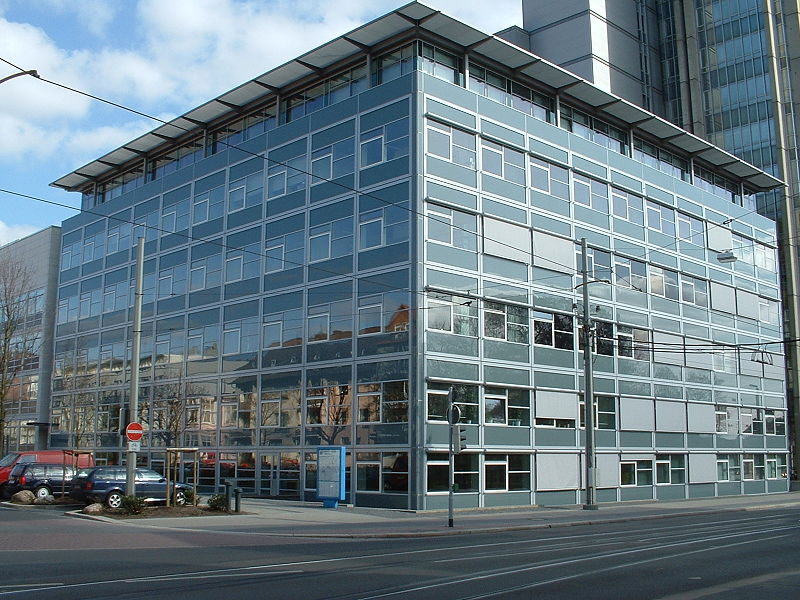
\includegraphics{infozentrum.jpg}}
\titlegraphic[scaled]{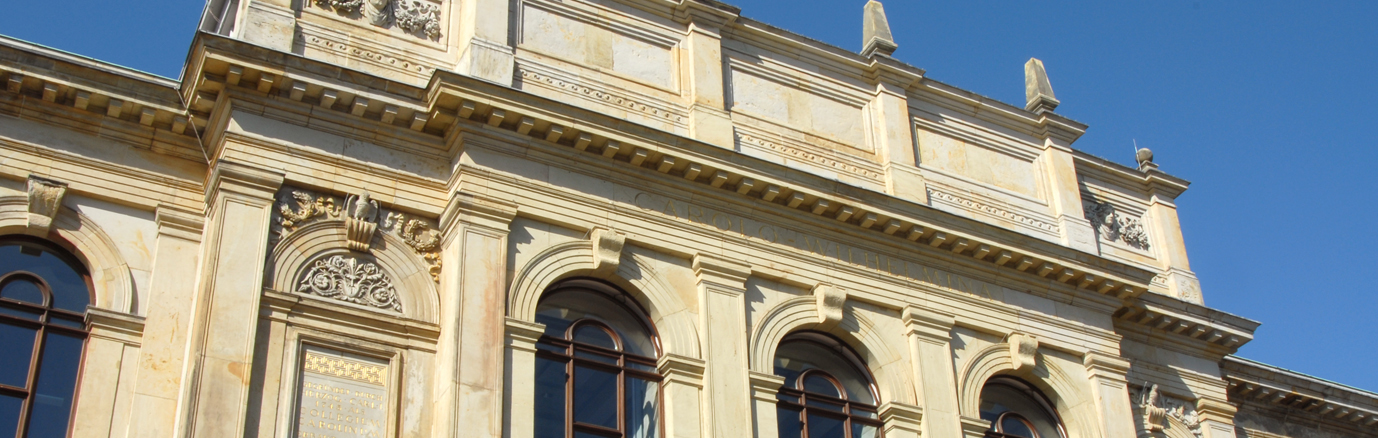
\includegraphics{titlepicture.jpg}}

% Logo, dass auf Titelseiten oben rechts und auf Inthaltsseiten unten rechts
% dargestellt wird. Es wird jeweils automatisch skliert
\logo{
\includegraphics{logo_wire_kreis.jpg}}
%\logo{Institut für Unkreativität\\und Schreibschwäche}

\begin{document}

\begin{frame}[plain]
\titlepage
\end{frame}

\begin{frame}{Inhalt}
\tableofcontents
\end{frame}


\section{The task}
\begin{frame}{Explaining the Task}
	\begin{itemize}
		\item extend an existing shallow water sovler
		\item with dynamic prallelism (DP)
	\end{itemize}
	\centering
	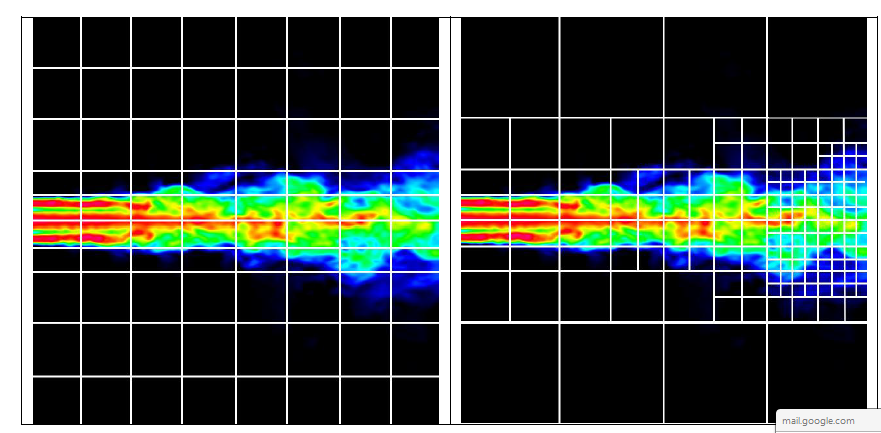
\includegraphics[width=0.8\textwidth]{dynamicparallelism.png}
\end{frame}

\section{Dynamic parallelism using CUDA}

\subsection{Implementation DP with CUDA}	
\begin{frame}[fragile]{Implementation DP with CUDA}
	\begin{itemize}
		\item DP in CUDA means calling a Kernel in a Kernal
		\item so every thread calls a new grid
	\end{itemize}

	\begin{verbatim}
		main(){
		    ...
		    <<< g,b >>> func(depth)
		}
	\end{verbatim}	

	\begin{verbatim}
		__global__ void func(int depth)
		{
		    if(depth<2)
		        func  <<< g, b >>> (depth+1)
		}
	\end{verbatim}
\end{frame}

\subsection{DP and Syncronisation}
\begin{frame}{DP and Syncronisation}
	\begin{itemize}
		\item One Kernel finished if his subkernel finished but it can work on after the supkernel call.
		\item To syncronize between one thread and his subkernels use cudaDeviceSynchronize() (this will not syncronize between threads)
	\end{itemize}
	\centering
	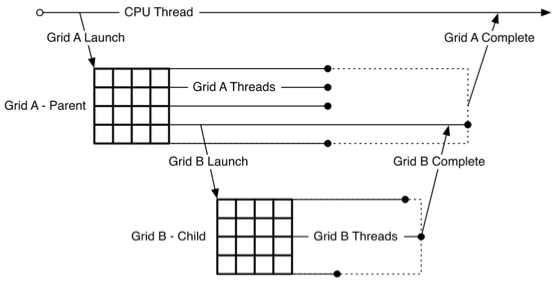
\includegraphics[width=0.8\textwidth]{nesting-of-grids.png}
\end{frame}


\subsection{Recursion Depth and Device Limits}
\begin{frame}[fragile]{Recursion Depth and Device Limits}
	\begin{itemize}
		\item nesting depth, limit to 24
			\begin{itemize}
				\item need to reserver buffer for running/suspended or launching kernels
				\item cudaDeviceSetLimit(cudaLimitDevRuntimePendingLaunchCount, x);
				\item default is set to 2048
			\end{itemize}
		\item synchronization depth
			\begin{itemize}
				\item cudaDeviceLimit(cudaLimitDevRuntimeSyncDepth, x)
				\item standart is 2
			\end{itemize}
	\end{itemize}
\end{frame}


\section{The Problem}
	\begin{frame}{Problem: Implemting of the datastructure}
		\begin{itemize}
			\item Datastructure: Forest (many Trees)
			\item Limit to getting coarse is the Forestsize (number of Trees)
			\item Limit to getting fine end up to the maximum recursions
			\item Trees: eg Quadtrees, Octrees...
		\end{itemize}		
	\end{frame}
\subsection{First try}

\begin{frame}[fragile]{With Pointer}
	\begin{verbatim}
			class LeafElem : public TreeElem
			{
			public:
  			float value;
  			__device__ __host__ LeafElem();
  			virtual __device__ __host__ ~LeafElem(){};
  			virtual __device__ __host__ bool isLeaf()
  			{
    			return true;
  			}
			};
	\end{verbatim}
\end{frame}

\begin{frame}[fragile]{With Pointer}
	\begin{verbatim}
			class BranchElem : public TreeElem
			{
			 public:
			    int nx;
			    int ny;
			    int depth;
			    TreeElem** children;
			    __device__ __host__ BranchElem(int nx, int ny, int depth);
			    virtual __device__ __host__ ~BranchElem();
			    virtual __device__ __host__ bool isLeaf()
			    {
			        return false;
			    }
			 };
	\end{verbatim}
\end{frame}

\begin{frame}{But this dont work}
\end{frame}

\subsection{Back to Arrays}
	\begin{frame}{Storing the Tree-Structure in an Array}
		\centering
		\begin{tabular}{ | c | c | c | c | c | c | c | c |}
			\hline
  			0 & 0 & 0 & 0 & 1 & 1 & 2 & 2 \\ \hline
  			0 & 0 & 0 & 0 & 1 & 1 & 2 & 2 \\ \hline
  			0 & 0 & 0 & 0 & 1 & 1 & 1 & 1 \\ \hline
			0 & 0 & 0 & 0 & 1 & 1 & 1 & 1 \\ \hline
  			0 & 0 & 0 & 0 & 0 & 0 & 0 & 0 \\ \hline
  			0 & 0 & 0 & 0 & 0 & 0 & 0 & 0 \\ \hline
  			0 & 0 & 0 & 0 & 0 & 0 & 0 & 0 \\ \hline
  			0 & 0 & 0 & 0 & 0 & 0 & 0 & 0 \\ \hline
		\end{tabular}
	\end{frame}
	
	\begin{frame}{Profiling}
		\centering
		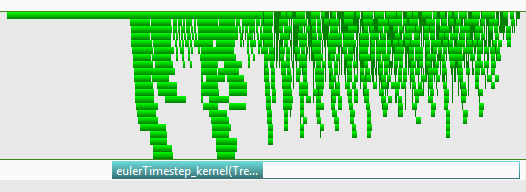
\includegraphics[width=1\textwidth]{profilingArray.png}
	\end{frame}



\end{document}
